\documentclass[12pt]{beamer}
\usepackage{../Estilos/BeamerMAF}
\input{../Preambulos/preambulo_Beamer_Warsaw_seahorse}
\makeatletter
\setbeamertemplate{footline}
{
  \leavevmode%
  \hbox{%
  \begin{beamercolorbox}[wd=.333333\paperwidth,ht=2.25ex,dp=1ex,center]{section in foot}%
    \usebeamerfont{section in foot} \insertsection
  \end{beamercolorbox}%
  \begin{beamercolorbox}[wd=.333333\paperwidth,ht=2.25ex,dp=1ex,center]{subsection in foot}%
    \usebeamerfont{subsection in foot}  \insertsubsection
  \end{beamercolorbox}%
  \begin{beamercolorbox}[wd=.333333\paperwidth,ht=2.25ex,dp=1ex,right]{date in head/foot}%
    \usebeamerfont{date in head/foot} \insertshortdate{} \hspace*{2em}
    \insertframenumber{} / \inserttotalframenumber \hspace*{2ex} 
  \end{beamercolorbox}}%
  \vskip0pt%
}
\makeatother
\makeatletter
\patchcmd{\beamer@sectionintoc}{\vskip1.5em}{\vskip0.8em}{}{}
\makeatother
\date{5 de marzo de 2021}
\title{Trabajando con vectores}
\subtitle{La física y la geometría}
\begin{document}
\maketitle
\fontsize{14}{14}\selectfont
\spanishdecimal{.}
\section*{Contenido}
\frame[allowframebreaks]{\tableofcontents[currentsection, hideallsubsections]}
\section{Introducción}
\frame[allowframebreaks]{\tableofcontents[currentsection, hideothersubsections]}
%Ref. Heinbockel (1996) Introduction to tensor calculus and continuum mechanics.
\subsection{Tipos de campos.}
\begin{frame}
\frametitle{Campos escalares y vectoriales}
Un campo escalar describe una correspondencia uno a uno entre un solo número escalar y un punto.
\\
\bigskip
\pause
Un campo vectorial de $n$ dimensiones se describe mediante una correspondencia biunívoca entre $n$ números y un punto. 
\end{frame}
\begin{frame}
\frametitle{Generalización}
Generalicemos estos conceptos asignando $n$ números al cuadrado a un solo punto o $n$ números al cubo a un solo punto.
\\
\bigskip
\pause
Cuando estos números obedecen a ciertas leyes de transformación, se convierten en ejemplos de campos tensoriales.
\end{frame}
\begin{frame}
\frametitle{Generalización}
En general, los campos escalares se denominan campos tensoriales de rango u orden cero, mientras que los campos vectoriales se denominan campos tensoriales de rango u orden uno.
\end{frame}

\section{Notación de índices}
\frame{\tableofcontents[currentsection, hideothersubsections]}
\subsection{Utilidad de los índices}

\begin{frame}
\frametitle{El uso de índices}
La notación indicial o de índices está estrechamente asociada con el cálculo tensorial.
\\
\bigskip
\pause
Resulta que los tensores tienen ciertas propiedades que son independientes del sistema de coordenadas utilizado para describir el tensor.
\end{frame}
\begin{frame}
\frametitle{El uso de índices}
Debido a estas útiles propiedades, podemos usar tensores para representar varias leyes fundamentales que ocurren en física, ingeniería, ciencia y matemáticas.
\\
\bigskip
\pause
Estas representaciones son extremadamente útiles ya que son independientes de los sistemas de coordenadas considerados.
\end{frame}
\subsection{Manejando los índices.}
\begin{frame}
\frametitle{Índices y vectores}
Dos vectores $\va{A}$ y $\va{B}$ se pueden presentar en una forma de sus componentes:
\begin{align*}
\va{A} &= A_{1} \, \vu{e}_{1} + A_{2} \, \vu{e}_{2} + A_{3} \, \vu{e}_{3} \\[0.5em]
\va{B} &= B_{1} \, \vu{e}_{1} + B_{2} \, \vu{e}_{2} + B_{3} \, \vu{e}_{3}
\end{align*}
donde $\vu{e}_{1}, \vu{e}_{2}$ y $\vu{e}_{3}$ son los vectores base ortogonales.
\end{frame}
\begin{frame}
\frametitle{Compactando la notación}
A menudo, cuando no surge ninguna confusión, los vectores $\va{A}$ y $\vu{B}$ se expresan en aras de la brevedad como números triples. Por ejemplo, podemos escribir:
\begin{align*}
\va{A} = A_{1} + A_{2} + A_{3} \hspace{1cm} \va{B} = B_{1} + B_{2} + B_{3}
\end{align*}
donde se sobreentiende que solamente se están indicando las componentes de los vectores $\va{A}$ y $\vu{B}$.
\end{frame}
\begin{frame}
\frametitle{Expresando vectores unitarios}
Los vectores unitarios se representarían como:
\begin{align*}
\vu{e}_{1} = (1, 0, 0), \hspace{1cm} \vu{e}_{2} = (0, 1, 0), \hspace{1cm} \vu{e}_{3} = (0, 0, 1)
\end{align*}
Una notación aún más corta, que representa los vectores $\va{A}$ y $\va{B}$, es la de índices o notación indicial.
\end{frame}
\begin{frame}
\frametitle{Notación de índices}
En la notación de índices, las cantidades
\begin{align*}
A_{i}, \hspace{0.5cm} i = 1, 2, 3 \hspace{1cm} \mbox{y} \hspace{1cm} B_{p}, \hspace{0.5cm} p = 1, 2, 3
\end{align*}
representan las componentes de los vectores $\va{A}$ y $\va{B}$.
\\
\bigskip
\pause
Esta notación enfoca la atención solo en los componentes de los vectores y emplea un \emph{subíndice ficticio (o mudo)} cuyo valor en los enteros está especificado.
\end{frame}
\begin{frame}
\frametitle{Notación de índices}
El símbolo $A_{i}$ se refiere a todos los componentes del vector $\va{A}$ de manera simultánea.
\\
\bigskip
\pause
El subíndice ficticio (o mudo) $i$ puede tener cualquiera de los valores enteros $1, 2$ o $3$.
\end{frame}
\begin{frame}
\frametitle{Notación de índices}
\setbeamercolor{item projected}{bg=blue!70!black,fg=yellow}
\setbeamertemplate{enumerate items}[circle]
\begin{enumerate}[<+->]
\item  Para $i = 1$ enfocamos la atención en el componente $A_{1}$ del vector $\va{A}$.
\item  Con $i = 2$ nos enfocamos en el segundo componente $A_{2}$ del vector $\va{A}$.
\item  Cuando $i = 3$ podemos centrar la atención en el tercer componente de $\va{A}$.
\end{enumerate}
\end{frame}
\begin{frame}
\frametitle{Notación de índices}
El subíndice $i$ es un subíndice mudo y puede ser reemplazado por otra letra, digamos $p$, siempre que se especifiquen los valores enteros que puede tener este subíndice mudo.
\end{frame}
\begin{frame}
\frametitle{Dimensiones mayores}
También es conveniente en este momento mencionar que los vectores de dimensiones superiores pueden definirse como $n$-tuplas ordenadas. Por ejemplo, el vector:
\begin{align*}
\va{X} = (X_{1}, X_{2}, \ldots, X_{N})
\end{align*}
con componentes $X_{i}, i =1, 2, \ldots, N$ es llamado un vector $N$-dimensional.
\end{frame}
\begin{frame}
\frametitle{Dimensiones mayores}
Otra notación que se utilizar para representar a este vector es:
\begin{align*}
\va{X} = X_{1} \, \vu{e}_{1} +  X_{2} \, \vu{e}_{2} +  \ldots +  X_{N} \, \vu{e}_{N}
\end{align*}
donde los
\begin{align*}
\vu{e}_{1}, \vu{e}_{2}, \ldots, \vu{e}_{N}
\end{align*}
son los vectores unitarios base linealmente independientes.
\end{frame}
\begin{frame}
\frametitle{Uso de notación de índices}
Tengamos en cuenta que muchas de las operaciones que ocurren en el uso de la notación de índices se aplican no solo a los vectores tridimensionales, sino también a los vectores $N$-dimensionales.
\end{frame}
\begin{frame}
\frametitle{Uso de notación de índices}
Más adelante será necesario definir cantidades que se pueden representar mediante una letra con subíndices o superíndices adjuntos. Estas cantidades se denominan sistemas. Cuando estas cantidades obedecen a ciertas leyes de transformación, se las denomina sistemas tensoriales. 
\end{frame}
\begin{frame}
\frametitle{Ejemplos de sistemas tensoriales}
Por ejemplo, cantidades como
\begin{align*}
&A_{ij}^{k} \hspace{0.5cm} e^{ijk} \hspace{0.5cm} \delta_{ij} \hspace{0.5cm} \delta_{i}^{j} \\[0.5em]
&A^{i} \hspace{0.5cm} B_{j} \hspace{0.5cm} a_{ij}
\end{align*}
\end{frame}
\begin{frame}
\frametitle{Reglas para índices}
Los subíndices o superíndices se denominan índices o sufijos. Cuando se presentan tales cantidades, los índices deben ajustarse a las siguientes reglas:
\setbeamercolor{item projected}{bg=blue!70!black,fg=yellow}
\setbeamertemplate{enumerate items}[circle]
\begin{enumerate}[<+->]
\item Son letras minúsculas latinas o griegas.
\item Las letras al final del alfabeto $(u, v, w, x, y, z)$ nunca se emplean como índices.
\end{enumerate}
\end{frame}
\begin{frame}
\frametitle{Orden de los sistemas}
El número de subíndices y superíndices determina el orden del sistema. \emph{Un sistema con un índice es un sistema de primer orden}.
\\
\bigskip
\pause
Un sistema con dos índices se denomina sistema de segundo orden. En general, un sistema con $N$ índices se denomina sistema de orden $N$. \pause Un sistema sin índices se denomina sistema de orden escalar o cero.
\end{frame}
\begin{frame}
\frametitle{Sistemas equivalentes}
El tipo de sistema depende del número de subíndices o superíndices que aparecen en una expresión.
\\
\bigskip
\pause
Por ejemplo: $A_{jk}^{i}$ y $B_{st}^{m}$ (todos los índices van de $1$ a $N$) son del mismo tipo porque tienen el mismo número de subíndices y superíndices.
\end{frame}
\begin{frame}
\frametitle{Sistemas equivalentes}
Por el contrario, los sistemas $A_{jk}^{i}$ y $C_{p}^{mn}$ no son del mismo tipo porque un sistema tiene solo tiene un superíndice y el otro sistema tiene dos superíndices.
\\
\bigskip
\pause
Para ciertos sistemas, el número de subíndices y superíndices es importante. En otros sistemas no tiene importancia.
\end{frame}
\begin{frame}
\frametitle{Aclaración importante}
En el uso de superíndices no se deben confundir las \enquote{potencias} de una cantidad con los superíndices.
\\
\bigskip
\pause
Por ejemplo, si reemplazamos las variables independientes $(x, y, z)$ por los símbolos $(x^{1}, x^{2}, x^{3})$, entonces estamos dejando $y = x^{2}$ donde $x^{2}$ es una variable y no $x$ elevado a una potencia.
\end{frame}
\begin{frame}
\frametitle{Aclaración importante}
De manera similar, la sustitución $z = x^{3}$ es el reemplazo de $z$ por la variable $x^{3}$ y esto no debe confundirse con $x$ elevado al cubo. 
\\
\bigskip
\pause
Para escribir una cantidad en superíndice a una potencia, usaremos paréntesis, por ejemplo, $(x^{2})^{3}$ es la variable $x^{2}$ al cubo.
\end{frame}
\begin{frame}
\frametitle{Relevancia de la notación}
Una de las razones para introducir las variables de superíndice \emph{es que se pueden hacer muchas ecuaciones de matemáticas y física para que adquieran una forma concisa y compacta}.
\end{frame}
\section{Convención en los índices}
\frame{\tableofcontents[currentsection, hideothersubsections]}
\subsection{Índices no repetidos}
\begin{frame}
\frametitle{Índices sin repetición}
Existe una convención de rango asociada con los índices. Esta convención establece que siempre que haya una expresión en la que los índices se presenten sin repetición, debe entenderse que cada uno de los subíndices o superíndices puede tomar cualquiera de los valores enteros $1,2, \ldots, N$ donde $N$ es un valor entero especificado.
\end{frame}
\begin{frame}
\frametitle{La delta de Kronecker}
Por ejemplo: la \emph{delta de Kronecker}, con símbolo $\delta_{ij}$, definida como
\begin{align*}
\delta_{ij} = \begin{cases}
1 & \mbox{si } i = j \\[0.5em]
0 & \mbox{si } i \neq j
\end{cases}
\end{align*}
con $i, j$ índices que recorren los valores $1, 2, 3$.
\end{frame}
\begin{frame}
\frametitle{La delta de Kronecker}
La delta de Kronecker representa nueve cantidades:
\begin{table}[H]
\large
\centering
\begin{tabular}{c c c}
$\delta_{11} = 1$ & $\delta_{12} = 0$ & $\delta_{13} = 0$ \\
$\delta_{21} = 0$ & $\delta_{22} = 1$ & $\delta_{23} = 0$ \\
$\delta_{31} = 0$ & $\delta_{32} = 0$ & $\delta_{33} = 1$
\end{tabular}
\end{table}
El símbolo $\delta_{ij}$ se refiere a todos los componentes del sistema de manera simultánea.
\end{frame}
\begin{frame}
\frametitle{Ejemplo de la delta}
Otro ejemplo, considera la ecuación:
\begin{align}
\vu{e}_{m} \cdot \vu{e}_{n} = \delta_{mn} \hspace{0.75cm} m, n = 1, 2, 3
\label{eq:ecuacion_01_01}
\end{align}
los subíndices $m, n$ aparecen sin repetición en el lado izquierdo de la ecuación y, por lo tanto, también deben aparecer en el lado derecho de la ecuación. \pause Estos índices se denominan índices \enquote{libres} y pueden tomar cualquiera de los valores $1, 2$ o $3$ según lo especificado por el rango.
\end{frame}
\begin{frame}
\frametitle{Ejemplo de la delta}
Dado que hay tres opciones para el valor de $m$ y tres opciones para un valor de $n$, encontramos que la ecuación (\ref{eq:ecuacion_01_01}) representa nueve ecuaciones simultáneamente. \pause Estas nueve ecuaciones son:
\begin{table}[H]
\large
\centering
\begin{tabular}{c c c}
$\vu{e}_{1} \cdot \vu{e}_{1} = 1$ & $\vu{e}_{1} \cdot \vu{e}_{2} = 0$ & $\vu{e}_{1} \cdot \vu{e}_{3} = 0$ \\
$\vu{e}_{2} \cdot \vu{e}_{1} = 0$ & $\vu{e}_{2} \cdot \vu{e}_{2} = 1$ & $\vu{e}_{2} \cdot \vu{e}_{3} = 0$ \\
$\vu{e}_{3} \cdot \vu{e}_{1} = 0$ & $\vu{e}_{3} \cdot \vu{e}_{2} = 0$ & $\vu{e}_{3} \cdot \vu{e}_{3} = 1$
\end{tabular}
\end{table}
\end{frame}

\section{Sistemas simétricos y asimétricos.}
\frame{\tableofcontents[currentsection, hideothersubsections]}
\subsection{Definiciones}

\begin{frame}
\frametitle{Sistema simétrico}
Se dice que un sistema definido por subíndices y superíndices que abarcan un conjunto de valores es simétrico en dos de sus índices si los componentes no cambian cuando se intercambian los índices.
\\
\bigskip
\pause
Por ejemplo, el sistema de tercer orden $T_{ijk}$ es simétrico en los índices $i$ y $k$ si
\begin{align*}
T_{ijk} = T_{kji} \hspace{1cm} \forall \hspace{0.2cm} i, j, k
\end{align*}
\end{frame}
\begin{frame}
\frametitle{Sistema asimétrico}
Se dice que un sistema definido por subíndices y superíndices es asimétrico en dos de sus índices, si los componentes cambian de signo cuando se intercambian los índices.
\\
\bigskip
\pause
Por ejemplo, el sistema de cuarto orden $T_{ijkl}$ es asimétrico en los índices $i$ y $l$ si
\begin{align*}
T_{ijkl} = -T_{ljki} \hspace{1cm} \forall \hspace{0.2cm} i, j, k
\end{align*}
\end{frame}
\begin{frame}
\frametitle{Ejemplo de asimetría}
Como otro ejemplo, considere el sistema de tercer orden $a_{prs}$, $p, r, s = 1, 2, 3$ que es completamente asimétrico en todos sus índices. \pause Entonces tendríamos:
\begin{align*}
a_{prs} = - a_{psr} = a_{spr} = -a_{srp} = a_{rsp} = -a_{rps}
\end{align*}
 Sería un buen ejercicio demostrar que este sistema completamente asimétrico tiene $27$ elementos, $21$ de los cuales son cero.
\end{frame}
\begin{frame}
\frametitle{Ejemplo de asimetría}
Los $6$ elementos distintos de cero están todos relacionados entre sí a través de las ecuaciones anteriores cuando $(p, r, s) = (1, 2, 3)$. 
\\
\bigskip
Esto se expresa diciendo que el sistema anterior tiene solo un componente independiente.
\end{frame}

\section{Convención de la suma}
\frame{\tableofcontents[currentsection, hideothersubsections]}
\subsection{Índices repetidos}

\begin{frame}
\frametitle{Convención de la suma}
La convención de suma establece que siempre que surge una expresión \emph{donde hay un índice que aparece dos veces en el mismo lado de cualquier ecuación, o término dentro de una ecuación, se entiende que representa una suma en estos índices repetidos}.
\end{frame}
\begin{frame}
\frametitle{Convención de la suma}
La suma está por encima de los valores enteros especificados por el rango. \emph{Un índice repetido se llama índice de suma}, mientras que \emph{un índice no repetido se llama índice libre.}
\\
\bigskip
\pause
La convención de suma requiere que nunca se debe permitir que un índice de suma aparezca más de dos veces en una expresión dada.
\end{frame}
\begin{frame}
\frametitle{Índices ficticios o mudos}
Debido a esta regla, a veces es necesario reemplazar un símbolo de suma ficticio (o mudo) por otro símbolo ficticio para evitar que aparezcan tres o más índices en el mismo lado de la ecuación.
\end{frame}
\begin{frame}
\frametitle{De nuevo la utilidad de los índices}
La notación de índices es una notación muy poderosa y se puede utilizar para representar de forma concisa muchas ecuaciones complejas. Esta notación se emplea para definir los componentes tensoriales y las operaciones asociadas con los tensores.
\end{frame}
\begin{frame}
\frametitle{Ejemplo 1}
Las siguientes dos ecuaciones
\begin{align*}
y_{1} &= a_{11} \, x_{1} + a_{12} \, x_{2} \\[0.5em]
y_{2} &= a_{21} \, x_{1} + a_{22} \, x_{2}
\end{align*}
se puede expresar como una sola ecuación al introducir un índice mudo, digamos $k$.
\end{frame}
\begin{frame}
\frametitle{Ejemplo 1}
Tal que las dos ecuaciones anteriores se pueden escribir como:
\begin{align*}
y_{k} = a_{k1} \, x_{1} + a_{k2} \, x_{2} \hspace{1cm} k = 1, 2
\end{align*}
La convención de rango establece que $k$ es libre de tener cualquiera de los valores $1$ o $2$ ($k$ es un índice libre).
\end{frame}
\begin{frame}
\frametitle{Ejemplo 1}
Esta ecuación ahora se puede escribir en la forma:
\begin{align*}
y_{k} = \sum_{i=1}^{2} a_{ki} \, x_{i} = a_{k1} \, x_{1} + a_{k2} \, x_{2}
\end{align*}
donde $i$ es el índice mudo de la suma.
\\
\bigskip
\pause
Cuando se retira la sigma que representa la suma y se ocupa la convención de la suma, se tiene que:
\begin{align*}
y_{k} = a_{ki} \, x_{i} , \hspace{1cm} i, k = 1, 2
\end{align*}
\end{frame}
\begin{frame}
\frametitle{Ejemplo 1}
Dado que el subíndice $i$ se repite, la convención de suma requiere que se realice una suma dejando que el subíndice de suma adopte los valores especificados por el rango y luego sumando los resultados. 
\end{frame}
\begin{frame}
\frametitle{Ejemplo 1}
El índice $k$ que aparece solo una vez a la izquierda y solo una vez a la derecha de la ecuación se llama índice libre. Cabe señalar que tanto $k$ como $i$ son subíndices ficticios y pueden reemplazarse por otras letras.
\\
\bigskip
\pause
Por ejemplo, podemos escribir:
\begin{align*}
y_{n} = a_{nm} \, x_{m} \hspace{1cm} n, m = 1, 2
\end{align*}
donde $m$ es el índice de suma y $n$ el índice libre.
\end{frame}
\begin{frame}
\frametitle{Ejemplo 1}
Sumando sobre $m$ se obtiene:
\begin{align*}
y_{n} = a_{n1} \, x_{1} + a_{n2} \, x_{2}
\end{align*}
y dejando que el índice libre $n$ tome los valores de $1$ y $2$, recuperamos las dos ecuaciones originales.
\end{frame}
\begin{frame}
\frametitle{Ejemplo 2}
Para $y_{i} = a_{ij} \, x_{j}$ con $i, j = 1, 2, 3$ y $x_{i} = b_{ij} \, z_{j}$ con $i, j = 1, 2, 3$, resolver para la variable $y$ en términos de la variable $z$.
\end{frame}
\begin{frame}
\frametitle{Ejemplo 2}
En una representación matricial, las dos ecuaciones anteriores se expresan como:
\fontsize{11}{11}\selectfont
\begin{align*}
\mqty(y_{1} \\ y_{2} \\ y_{3}) = \mqty(
a_{11} & a_{12} & a_{13} \\
a_{21} & a_{22} & a_{23} \\
a_{31} & a_{32} & a_{33}
) \, \mqty(
x_{1} \\ x_{2} \\ x_{3}
) \\[1em]
\mqty(x_{1} \\ x_{2} \\ x_{3}) = \mqty(
b_{11} & b_{12} & b_{13} \\
b_{21} & b_{22} & b_{23} \\
b_{31} & b_{32} & b_{33}
) \, \mqty(
z_{1} \\ z_{2} \\ z_{3}
)
\end{align*}
\end{frame}
\begin{frame}
\frametitle{Ejemplo 2}
Para resolver $y$ en términos de la variable $z$, tendremos que:
\begin{align*}
\mqty(y_{1} \\ y_{2} \\ y_{3}) = \mqty(
a_{11} & a_{12} & a_{13} \\
a_{21} & a_{22} & a_{23} \\
a_{31} & a_{32} & a_{33}
) \, \mqty(
b_{11} & b_{12} & b_{13} \\
b_{21} & b_{22} & b_{23} \\
b_{31} & b_{32} & b_{33}
) \, \mqty(
z_{1} \\ z_{2} \\ z_{3}
)        
\end{align*}
\end{frame}
\begin{frame}
\frametitle{Ejemplo 2}
La notación de índices emplea índices que son índices mudos, por lo que podemos escribir:
\begin{align*}
y_{n} &= a_{nm} \, x_{m}, \hspace{0.5cm} n, m = 1, 2, 3 \\[0.5em]
x_{m} &= b_{mj} \, z_{j}, \hspace{0.5cm} m, j = 1, 2, 3
\end{align*}
\pause
Aquí hemos cambiado deliberadamente los índices de modo que cuando sustituimos $x_{m}$, de una ecuación a la otra, un índice de suma no se repite más de dos veces.
\end{frame}
\begin{frame}
\frametitle{Ejemplo 2}
Sustituyendo encontramos la forma en índices de la ecuación matricial anterior como:
\begin{align*}
y_{n} = a_{nm} \, b_{mj} \, z_{j} \hspace{0.5cm} m, n, j = 1, 2, 3
\end{align*}
donde $n$ es el índice libre y $m$, $j$ son los índices mudos para la suma.
\end{frame}
% \par
% \noindent
% \textbf{Ejemplo: } El producto punto de dos vectores $A_{q}$ con $q = 1, 2, 3$ y $B_{j}$, con $j = 1, 2, 3$, se representa con la notación de índices como:
% \begin{align*}
% A_{i} \, B_{i} = A \, B \, \cos \theta \hspace{0.75cm} i = 1, 2, 3, \hspace{0.75cm} A = \abs{\va{A}}, \hspace{0.3cm} B = \abs{\va{B}}
% \end{align*}
% Ya que el índice $i$ está repetido, se entiende que representa el índice de la suma. Al sumar sobre $i$ en el rango indicado, tenemos:
% \begin{align*}
% A_{1} \, B_{1} + A_{2} \, B_{2} + A_{3} \, B_{3} = A \, B \, \cos \theta
% \end{align*}
% Veamos que la notación de índices emplea índices ficticios. En ocasiones, estos índices se modifican para ajustarse a las reglas de suma anteriores, sin que se preste atención al cambio. Como en este ejemplo, los índices $q$ y $j$ son índices ficticios y se pueden cambiar a otras letras si se desea. Además, si no se indica el rango de los índices, se asume que el rango está por encima de los valores enteros 1, 2 y 3.
% \par
% A los sistemas que contienen subíndices y superíndices se pueden aplicar ciertas operaciones algebraicas. Presentamos a continuación de manera informal las operaciones de suma, multiplicación y contracción.

\section{Suma, multiplicación y contracción.}
\frame{\tableofcontents[currentsection, hideothersubsections]}
\subsection{Definiciones}

\begin{frame}
\frametitle{La suma}
La operación algebraica de suma o resta se aplica a sistemas del mismo tipo y orden.
\\
\bigskip
\pause
Es decir, podemos sumar o restar componentes similares en sistemas. Por ejemplo, la suma de $A_{jk}^{i}$ y $B_{jk}^{i}$ es nuevamente un sistema del mismo tipo y se denota por $C_{jk}^{i} = A_{jk}^{i} + B_{jk}^{i}$, donde se suman componentes similares.
\end{frame}
\begin{frame}
\frametitle{El producto}
El producto de dos sistemas se obtiene multiplicando cada componente del primer sistema por cada componente del segundo sistema.
\\
\bigskip
\pause
Tal producto se llama \emph{producto externo}.
\end{frame}
\begin{frame}
\frametitle{Orden del producto}
El orden del sistema de producto resultante es la suma de los órdenes de los dos sistemas involucrados en la formación del producto.
\\
\bigskip
\pause
Por ejemplo, si $A_{j}^{i}$ es un sistema de segundo orden y $B^{mnl}$ es un sistema de tercer orden, con todos los índices que tienen el rango de $1$ a $N$, entonces el sistema de productos es de quinto orden y se denota $C_{j}^{imnl} = A_{j}^{i} \, B^{mnl}$.
\end{frame}
\begin{frame}
\frametitle{Orden del producto}
El sistema obtenido por el producto representa $N^{5}$ términos construidos a partir de todos los productos posibles de los componentes de $A_{j}^{i}$ con los componentes de $B^{mnl}$.
\end{frame}
\begin{frame}
\frametitle{La contracción}
La operación de contracción se produce cuando un índice inferior se iguala a un índice superior y se invoca la convención de suma.
\end{frame}
\begin{frame}
\frametitle{La contracción}
Por ejemplo, si tenemos un sistema de quinto orden $C_{j}^{imnl}$ y hacemos que $i = j$ para luego hacer la suma, entonces hemos formado el sistema:
\begin{align*}
C^{mnl} = C_{j}^{jmnl} = C_{1}^{1mnl} + C_{2}^{2mnl} + \ldots + C_{N}^{Nmnl}
\end{align*}
Aquí el símbolo $C^{mnl}$ se usa para representar el sistema de tercer orden que resulta cuando se realiza la contracción.
\end{frame}
\begin{frame}
\frametitle{Orden de la contracción}
Siempre que se realiza una contracción, el sistema resultante es siempre de orden $2$ veces menor que el sistema original.
\\
\bigskip
\pause
Bajo ciertas condiciones especiales, está permitido realizar una contracción en dos índices minúsculas. 
\end{frame}

\section{La e-permutación y la \texorpdfstring{$\delta$}{d} de Kronecker}
\frame{\tableofcontents[currentsection, hideothersubsections]}
\subsection{Definiciones}

\begin{frame}
\frametitle{El símbolo e-permutación}
El símbolo de e-permutación a veces se denomina \emph{tensor alterno}.
\\
\bigskip
El símbolo de e-permutación, como su nombre indica, se ocupa de las permutaciones.
\end{frame}
\begin{frame}
\frametitle{Las permutaciones}
Una permutación es un arreglo de cosas. Cuando se cambia el orden de la disposición, se produce una nueva permutación.
\\
\bigskip
\pause
Una transposición es un intercambio de dos términos consecutivos en un arreglo.
\end{frame}
\begin{frame}
\frametitle{Ejemplo de permutación}
Como ejemplo, cambiemos los dígitos $1 \, 2 \, 3$ a $3 \, 2 \, 1$ haciendo una secuencia de transposiciones.
\\
\bigskip
\pause
\setbeamercolor{item projected}{bg=blue!70!black,fg=yellow}
\setbeamertemplate{enumerate items}[circle]
\begin{enumerate}[<+->]
\item Comenzando con los dígitos en el orden $1 \, 2 \, 3$ intercambiamos $2$ y $3$ (primera transposición) para obtener $1 \, 3 \, 2$. \item Luego, intercambiamos los dígitos $1$ y $3$ (segunda transposición) para obtener $3 \, 1 \, 2$.
\item Finalmente, intercambia los dígitos $1$ y $2$ (tercera transposición) para lograr $3 \, 2 \, 1$. 
\end{enumerate}
\end{frame}
\begin{frame}
\frametitle{Transposiciones}
Aquí el número total de transposiciones de $1 \, 2 \, 3$ a $3 \, 2 \, 1$ es tres, un número impar.
\\
\bigskip
\pause
También se pueden escribir otras transposiciones de $1 \, 2 \, 3$ a $3 \, 2 \, 1$. Sin embargo, también se trata de un número impar de transposiciones.
\end{frame}
\begin{frame}
\frametitle{Ejemplo 3}
El número total de formas posibles de ordenar los dígitos $1 \, 2 \, 3$ es seis.
\\
\bigskip
\pause
Tenemos tres opciones para el primer dígito. Habiendo elegido el primer dígito, solo quedan dos opciones para el segundo dígito. Por tanto, el número restante corresponde al último dígito.
\end{frame}
\begin{frame}
\frametitle{Ejemplo 3}
El producto $(3) (2) (1) = 3! = 6$ es el número de permutaciones de los dígitos $1$, $2$ y $3$. Estas seis permutaciones son:
\fontsize{11}{11}\selectfont
\begin{table}[H]
\centering
\begin{tabular}{c l}
$1 \, 2 \, 3$ & permutación par \\
$1 \, 3 \, 2$ & permutación impar \\
$3 \, 1 \, 2$ & permutación par \\
$3 \, 2 \, 1$ & permutación impar \\
$2 \, 3 \, 1$ & permutación par \\
$2 \, 1 \, 3$ & permutación impar \\
\end{tabular}
\end{table}
\end{frame}
\begin{frame}
\frametitle{Permutaciones pares o impares}
Aquí, una permutación de $1 \, 2 \, 3$ se llama par o impar dependiendo de si hay un número par o impar de transposiciones de los dígitos. 
\\
\bigskip
En la figura (\ref{fig:figura_01_01}) se ilustra una regla mnemónica para recordar las permutaciones pares e impares de $1 \, 2 \, 3$. 
\end{frame}
\begin{frame}
\frametitle{Permutaciones pares o impares}
\begin{figure}[H]
\centering
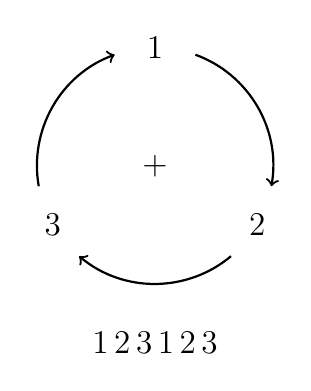
\begin{tikzpicture}[thick, scale=1.5, font=\large]
    \node (i) at (90:1cm)  {$1$};
    \node (j) at (-30:1cm) {$2$};
    \node (k) at (210:1cm) {$3$};
 
    \draw [->] (70:1cm)  arc (70:-10:1cm);
    \draw [->] (-50:1cm) arc (-50:-130:1cm);
    \draw [->] (190:1cm) arc (190:110:1cm);

    \node at (0, 0) {$\mathbf{+}$};
    \node at (0, -1.5) {$1 \, 2 \, 3 \, 1 \, 2 \, 3$};
\end{tikzpicture}
\hspace{2cm}
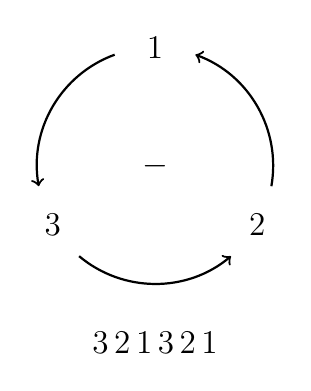
\begin{tikzpicture}[thick, scale=1.5, font=\large]
    \node (i) at (90:1cm)  {$1$};
    \node (j) at (-30:1cm) {$2$};
    \node (k) at (210:1cm) {$3$};
 
    \draw [<-] (70:1cm)  arc (70:-10:1cm);
    \draw [<-] (-50:1cm) arc (-50:-130:1cm);
    \draw [<-] (190:1cm) arc (190:110:1cm);

    \node at (0, 0) {$\mathbf{-}$};
    \node at (0, -1.5) {$3 \, 2 \, 1 \, 3 \, 2 \, 1$};
\end{tikzpicture}
\caption{Permutaciones de $1 \, 2 \, 3$.}
\label{fig:figura_01_01}
\end{figure}
\end{frame}
\begin{frame}
\frametitle{Permutaciones pares e impares}
Tengamos en cuenta que las permutaciones pares de $1 \, 2 \, 3$ se obtienen seleccionando tres números consecutivos cualesquiera de la secuencia $1 \, 2 \, 3\, 1 \, 2 \, 3$.
\\
\bigskip
\pause
Las permutaciones impares resultan seleccionando tres números consecutivos cualesquiera de la secuencia $3 \, 2 \, 1 \, 3 \, 2 \, 1$.
\end{frame}
\begin{frame}
\frametitle{Número de permutaciones}
 En general, el número de permutaciones de $n$ cosas tomadas de $m$, una a la vez, está dada por la relación:
\begin{align*}
P(n, m) = n (n - 1)(n - 2) \ldots (n - m +1)
\end{align*}
Al seleccionar un subconjunto de $m$ objetos de una colección de $n$ objetos, donde $m \leq n$, sin tener en cuenta el orden, se llama una combinación de $n$ objetos tomados $m$ a la vez.
\end{frame}
\begin{frame}
\frametitle{Número de permutaciones}
Por ejemplo, las combinaciones de $3$ números tomados del conjunto \\ $\left\{ 1, 2, 3, 4 \right\}$ son $(123), (124), (134), (234)$. Tomemos en cuenta que no se considera una combinación.
\\
\bigskip
\pause
Es decir, las permutaciones
\begin{align*}
(123), (132), (231), (213), (312), (321)
\end{align*}
se consideran iguales.
\end{frame}
\begin{frame}
\frametitle{Número de permutaciones}
En general, el número de combinaciones de $n$ objetos tomados de $m$ uno a la vez, está dada por:
\begin{align*}
C(n, m) = \binom{n}{m} = \dfrac{n!}{m! \, (n - m)!}
\end{align*}
La definición de permutaciones puede utilizarse para definir el símbolo de la e-permutación.
\end{frame}
\begin{frame}[fragile]
\frametitle{Definición de e-permutación}
\fbox{%
    \parbox{\textwidth}{%
  El símbolo de e-permutación (o tensor alternante) se define por:
\fontsize{11}{11}\selectfont
    \begin{align*}
    e^{ijk \ldots l} = e_{ijk \ldots l} = \begin{cases}
        1 & \mbox{si } ijk \ldots l \mbox{ es una p. par de } 1 2 3 \ldots n \\
        -1 & \mbox{si } ijk \ldots l \mbox{ es una p. impar de } 1 2 3 \ldots n \\
        0 & \mbox{en todos los otros casos}
    \end{cases}
    \end{align*}
    }%
}
\end{frame}
\begin{frame}
\frametitle{Ejemplo 4}
Calcula $e_{612453}$.
\\
\bigskip
\pause
Para determinar si $612453$ es una permutación par o impar de $123456$, escribimos los números dados y debajo de ellos escribimos los números enteros del $1$ al $6$.
\end{frame}
\begin{frame}
\frametitle{Ejemplo 4}
Luego, los números iguales se conectan mediante una línea:
\begin{figure}[H]
\centering
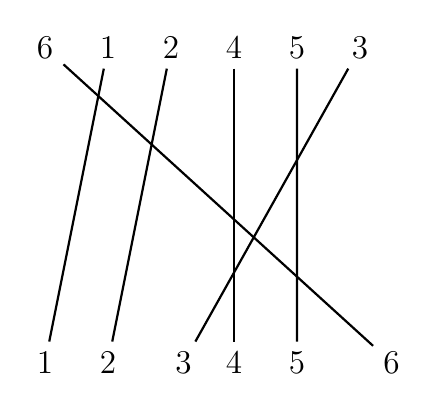
\begin{tikzpicture}[scale=0.8, thick, font=\large]
\node (A1) at (0, 0) {$6$};
\node (B1) at (1, 0) {$1$};
\node (C1) at (2, 0) {$2$};
\node (D1) at (3, 0) {$4$};
\node (E1) at (4, 0) {$5$};
\node (F1) at (5, 0) {$3$}; \pause

\node (A2) at (0, -5) {$1$};
\node (B2) at (1, -5) {$2$};
\node (C2) at (2.2, -5) {$3$};
\node (D2) at (3, -5) {$4$};
\node (E2) at (4, -5) {$5$};
\node (F2) at (5.5, -5) {$6$}; \pause

\draw (A1) -- (F2); \pause
\draw (B1) -- (A2); \pause
\draw (C1) -- (B2); \pause
\draw (D1) -- (D2); \pause
\draw (E1) -- (E2); \pause
\draw (F1) -- (C2); \pause
\end{tikzpicture}
\caption{Permutaciones de $123456$}
\label{fig:figura_01_02}
\end{figure}
\end{frame}
\begin{frame}
\frametitle{Total de cruces entre líneas}
En la figura (\ref{fig:figura_01_02}) hay siete intersecciones de las líneas que conectan números iguales.
\\
\bigskip
\pause
El número de intersecciones es un número impar y muestra que se debe realizar un número impar de transposiciones.
\\
\bigskip
\pause
Estos resultados implican que $e_{612453} = -1$
\end{frame}
\begin{frame}
\frametitle{La delta de Kronecker}
Otra definición utilizada con bastante frecuencia en la representación de cantidades matemáticas y de ingeniería es el delta de Kronecker, que ahora definimos en términos de subíndices y superíndices:
\end{frame}
\begin{frame}
\frametitle{La delta de Kronecker}
\noindent\fbox{%
    \parbox{0.9\textwidth}{%
    \textbf{Definición: } La delta de Kronecker está definida como:
    \begin{align*}
    \delta_{ij} = \delta_{i}^{j} = \begin{cases}
        1 & \mbox{si } i = j \\
        0 & \mbox{si } i \neq j
    \end{cases}
    \end{align*}
    }%
}
\end{frame}
% \\[1em]
% \noindent
% \textbf{Ejemplo: } Algunos ejemplos del símbolo de e-permutación y de la delta de Kronecker son:
% \begin{table}[H]
% \large
% \centering
% \begin{tabular}{l c c}
% $e_{123} = e^{123} = +1$ & $\delta_{1}^{1} =  1$ & $\delta_{12} = 0$ \\
% $e_{213} = e^{213} = -1$ & $\delta_{2}^{1} =  0$ & $\delta_{22} = 1$ \\
% $e_{112} = e^{112} = 0$ & $\delta_{3}^{1} =  0$ & $\delta_{32} = 0$
% \end{tabular}
% \end{table}

% \noindent
% \textbf{Ejemplo:} Cuando un índice de la delta de Kronecker $\delta_{ij}$ está involucrado en la convención de suma, el efecto es el de reemplazar un índice con un índice diferente. Por ejemplo, denotemos $a_{ij}$ los elementos de una matriz $N \times N$. Aquí se permite que $i$ y $j$ oscilen sobre los valores enteros $1, 2, \ldots , N$. Considera el producto
% \begin{align*}
% a_{ij} \, \delta_{ik}
% \end{align*}
% donde el rango de $i, j, k$ es $1, 2, \ldots , N$. El índice $i$ se repite y por lo tanto se entiende que representa una suma en el rango. El índice $i$ se llama índice de suma. Los otros índices $j$ y $k$ son índices libres. Son libres de que se les asigne cualquier valor del rango de los índices. No están involucrados en ninguna suma y sus valores, independientemente de lo que elija asignarles, son fijos. Asignemos un valor de $\underline{j}$ y $\underline{k}$ a los valores de $j$ y $k$. El guión bajo es para recordarle que estos valores para $j$ y $k$ son fijos y no se deben sumar. Cuando realizamos la suma sobre el índice de suma $i$, asignamos valores a $i$ del rango y luego sumamos sobre estos valores. Realizando la suma indicada obtenemos:
% \begin{align*}
% a_{i \underline{j}} \, \delta_{i \underline{k}} = a_{1 \underline{j}} \, \delta_{1 \underline{k}} + a_{2 \underline{j}} \, \delta_{2 \underline{k}} + \ldots + a_{\underline{k} \, \underline{j}} \, \delta_{\underline{k} \, \underline{k}} + \ldots + a_{N \underline{j}} \, \delta_{N \underline{k}}
% \end{align*}
% En esta suma, el delta de Kronecker es cero en todos los lugares donde los subíndices son diferentes y es igual a uno cuando los subíndices son iguales. Solo hay un término en esta suma que es distinto de cero. Es ese término donde el índice de suma $i$ era igual al valor fijo $k$ Esto da el resultado:
% \begin{align*}
% a_{\underline{k} \, \underline{j}} \, \delta_{k \, k} = a_{\underline{k} \, \underline{j}}
% \end{align*}
% donde el subrayado es para recordar que las cantidades tienen valores fijos y no se deben sumar. Quitando los guiones bajos que escribimos:
% \begin{align*}
% a_{ij} \, \delta_{i k} = a_{k j}
% \end{align*}
% Aquí hemos sustituido el índice $i$ por $k$, por lo que cuando se usa el delta de Kronecker en un proceso de suma, se lo conoce como operador de sustitución. Esta propiedad de sustitución del delta de Kronecker se puede utilizar para simplificar una variedad de expresiones que involucran la notación de índice. Algunos ejemplos son:
% \begin{align*}
% B_{ij} \, \delta_{js} &= B_{is} \\[0.5em]
% \delta_{jk} \, \delta_{km} = \delta_{jm} \\[0.5em]
% e_{ijk} \, \delta_{im} \, \delta_{jn} \, \delta_{kp} = e_{mnp}
% \end{align*}
% Algunos textos adoptan la notación de que si los índices son letras mayúsculas, no se debe realizar ninguna suma. Por ejemplo:
% \begin{align*}
% a_{KJ} \, \delta_{KK} = a_{KJ}
% \end{align*}
% ya que $\delta_{KK}$ representa un solo término debido a las letras mayúsculas. Otra notación que se utiliza para indicar que no hay suma de los índices es poner paréntesis sobre los índices que no se van a sumar. Por ejemplo,
% \begin{align*}
% a_{(k) j} \, \delta_{(k) (k)} = a_{kj}
% \end{align*}
% dado que $\delta_{(k) (k)}$ representa un solo término y los paréntesis indican que no se debe realizar ninguna suma. En cualquier momento podemos emplear la notación de subrayado, la notación de letras mayúsculas o la notación de paréntesis para indicar que no se debe realizar ninguna suma de los índices. Para evitar confusiones por completo, se pueden escribir expresiones entre paréntesis como \enquote{(no sumar sobre $k$)}.
% \\[0.5em]
% \noindent
\begin{frame}
\frametitle{Ejemplo 5}
En el símbolo delta de Kronecker $\delta_{j}^{i}$ hacemos $j$ igual a $i$, para luego hacer la suma. \emph{Esta operación se llama contracción}.
\\
\bigskip
\pause
Se obtiene como resultado $\delta_{i}^{i}$, que se suma en el rango del índice $i$.
\end{frame}
\begin{frame}
\frametitle{Ejemplo 5}
Utilizando el rango $1, 2, \ldots, N$ tenemos:
\begin{eqnarray*}
\delta_{i}^{i} &=& \delta_{1}^{1} + \delta_{2}^{2} + \ldots + \delta_{N}^{N} \\[0.5em] \pause
\delta_{i}^{i} &=& 1 + 1 + \ldots +  1 \\[0.em] \pause
\delta_{i}^{i} &=& N
\end{eqnarray*}
\end{frame}
\begin{frame}
\frametitle{En más dimensiones}
En tres dimensiones tenemos $\delta_{j}^{i}$ con $i, j = 1, 2, 3$ y
\begin{align*}
\delta_{k}^{k} = \delta_{1}^{1} + \delta_{2}^{2} + \delta_{3}^{3} = 3
\end{align*}
\end{frame}
\begin{frame}
\frametitle{Casos especiales}
En determinadas circunstancias, la delta de Kronecker se puede escribir solo con subíndices. Por ejemplo, $\delta_{ij}$ con $i, j = 1, 2, 3$.
\\
\bigskip
Encontraremos que estas circunstancias nos permiten realizar una contracción en los índices inferiores, de modo que $\delta_{ii} = 3$.
\end{frame}
\begin{frame}
\frametitle{Ejemplo 6}
El determinante de una matriz $A = (a_{ij})$ se puede expresar con notación de índices.
\\
\bigskip
\pause
Ocupando el símbolo de e-permutación, el determinante de una matriz de $N \times N$ se expresa como:
\begin{align*}
\abs{A} = e_{ij \ldots k} \, a_{1i} \, a_{2j} \, \ldots \, a_{Nk} 
\end{align*}
donde $e_{ij \ldots k}$ es un sistema de orden $N$.
\end{frame}
\begin{frame}
\frametitle{Ejemplo 6. Matriz de $2 \times 2$}
En el caso especial de una matriz de $2 \times 2$, escribimos:
\begin{align*}
\abs{A} = e_{ij} \, a_{1i} \, a_{2j}
\end{align*}
donde la suma se realiza en el rango $1, 2$, y el símbolo de e-permutación es de orden $2$.
\end{frame}
\begin{frame}
\frametitle{Ejemplo 6. Matriz de $3 \times 3$}
{\fontsize{12}{12}\selectfont En el caso especial de una matriz de $3 \times 3$, se tiene que:}
\begin{align*}
\abs{A} = \mqty|
a_{11} & a_{12} & a_{13} \\
a_{21} & a_{22} & a_{23} \\
a_{31} & a_{32} & a_{33}
| = e_{ijk} \, a_{i1} \, a_{j2} \, a_{k3} {=} e_{ijk} \, a_{1i} \, a_{2j} \, a_{3k}
\end{align*}
{\fontsize{12}{12}\selectfont
donde $i, j, k$ son los índices de suma y la suma está en el rango $1, 2, 3$.}
\end{frame}
\begin{frame}
\frametitle{Ejemplo 6. Matriz de $3 \times 3$}
El $e_{ijk}$ denota el símbolo de e-permutación de orden $3$.
\\
\bigskip
\pause
Tengamos en cuenta que al intercambiar las filas de la matriz de $3 \times 3$ podemos obtener resultados más generales.
\end{frame}
\begin{frame}
\frametitle{El determinante}
Consideremos $(p, q, r)$ una permutación de los enteros $(1, 2, 3)$ y veamos que el determinante se puede expresar como:
\begin{align*}
\Delta = \mqty|
a_{p1} & a_{p2} & a_{p3} \\
a_{q1} & a_{q2} & a_{q3} \\
a_{r1} & a_{r2} & a_{r3}
| = e_{ijk} \, a_{p1} \, a_{q2} \, a_{r3}
\end{align*}
\end{frame}
\begin{frame}
\frametitle{El determinante}
Para la secuencia $(1, 2, 3)$:
\fontsize{12}{12}\selectfont
\begin{table}[H]
\large
\centering
\begin{tabular}{l}
Si $(p, q, r)$ es una p. par $\Rightarrow \Delta = \abs{A}$ \\
Si $(p, q, r)$ es una p. impar $\Rightarrow \Delta = -\abs{A}$ \\
Si $(p, q, r)$ no es una p. $\Rightarrow \Delta = 0$    
\end{tabular}
\end{table}
\end{frame}
\begin{frame}
\frametitle{El determinante}
Entonces podemos escribir:
\begin{align*}
e_{ijk} \, a_{pi} \, a_{qj} \, a_{rk} = e_{pqr} \, \abs{A}
\end{align*}
\end{frame}
\begin{frame}
\frametitle{Ejemplo 7}
La expresión $e_{ijk} \, B_{ij} \, C_{i}$ no tiene sentido ya que el índice $i$ se repite más de dos veces y la convención de suma no lo permite.
\\
\bigskip
\pause
Si realmente se deseaba sumar sobre un índice que ocurre más de dos veces, entonces debe usarse un signo de suma.
\end{frame}
\begin{frame}
\frametitle{Ejemplo 7}
Por ejemplo, la expresión anterior sería:
\begin{align*}
\sum_{i=1}^{n} e_{ijk} \, B_{ij} \, C_{i}
\end{align*}
\end{frame}
\begin{frame}
\frametitle{Ejemplo 8}
El producto cruz de los vectores unitarios $\vu{e}_{1}, \vu{e}_{2}, \vu{e}_{3}$ y con la secuencia $(1, 2, 3)$ se puede expresar en notación de índices como: 
\begin{align*}
\vu{e}_{i} \times \vu{e}_{j} = \begin{cases}
\vu{e}_{k} & \mbox{si } (i, j, k) \mbox{ es una p. par} \\
-\vu{e}_{k} & \mbox{si } (i, j, k) \mbox{ es una p. impar} \\
0 & \mbox{para todos los demás casos}
\end{cases}
\end{align*}
\end{frame}
\begin{frame}
\frametitle{Ejemplo 8}
Este resultado se puede escribir de la forma:
\begin{align*}
\vu{e}_{i} \times \vu{e}_{j} = e_{kij} \, \vu{e}_{k}
\end{align*}
Este último resultado se puede verificar sumando sobre l índice $k$ y escribir las $9$ combinaciones posibles para $i$ y $j$.
\end{frame}
\begin{frame}
\frametitle{Ejemplo 9}
Dados los vectores $A_{p}$, con $p = 1, 2, 3$ y $B_{p}$ con $p = 1, 2, 3$ el producto cruz de los dos vectores es un vector $C_{p}$ con $p = 1, 2, 3$, con componentes:
\begin{align}
C_{i} = e_{ijk} \, A_{j} \, B_{k} \hspace{1cm} i, j, k = 1, 2, 3
\label{eq:ecuacion_01_02}
\end{align}
\end{frame}
\begin{frame}
\frametitle{Ejemplo 9}
Donde las cantidades $C_{i}$ representan las componentes del vector producto cruz:
\begin{align*}
\va{C} = \va{A} \cp \va{B} = C_{1} \, \vu{e}_{1} + C_{2} \, \vu{e}_{2} + C_{3} \, \vu{e}_{3} 
\end{align*}
\end{frame}
\begin{frame}
\frametitle{Ejemplo 9}
La ec. (\ref{eq:ecuacion_01_02}) define las componentes de $\va{C}$, se sumará en cada uno de los índices que
se repite.
\\
\bigskip
\pause
Sumando sobre el índice $k$:
\begin{align}
C_{i} = e_{ij1} \, A_{j} \, B_{1} + e_{ij2} \, A_{j} \, B_{2} + e_{ij3} \, A_{j} \, B_{3}
\label{eq:ecuacion_01_03}     
\end{align}
\end{frame}
\begin{frame}
\frametitle{Ejemplo 9}
La siguiente suma sobre el índice $j$ el cual se repite en cada término de la ecuación (\ref{eq:ecuacion_01_03}), obteniendo:
\begin{align}
\begin{aligned}
C_{i} &= e_{i11} \, A_{1} \, B_{1} + e_{i21} \, A_{2} \, B_{1} + e_{i31} \, A_{3} \, B_{1} \, + \\[0.5em]
&+ e_{i12} \, A_{1} \, B_{2} + e_{i22} \, A_{2} \, B_{2} + e_{i32} \, A_{3} \, B_{2} \, + \\[0.5em]
&+ e_{i13} \, A_{1} \, B_{3} + e_{i23} \, A_{2} \, B_{3} + e_{i33} \, A_{3} \, B_{3}
\end{aligned}
\label{eq:ecuacion_01_04}
\end{align}
\end{frame}
\begin{frame}
\frametitle{Ejemplo 9}
Ahora nos quedamos con $i$ como un índice libre que puede tener cualquiera de los valores de $1, 2$ o $3$. Dejando que $i = 1$, luego dejando $i = 2$, y finalmente dejando que $i = 3$ produce los componentes del producto cruz:
\begin{align*}
C_{1} &= A_{2} \, B_{3} - A_{3} \, B_{2} \\[0.5em]
C_{2} &= A_{3} \, B_{1} - A_{1} \, B_{3} \\[0.5em]
C_{3} &= A_{1} \, B_{2} - A_{2} \, B_{1}
\end{align*}
\end{frame}
\begin{frame}
\frametitle{Ejemplo 9}
El producto cruz también puede expresarse de la forma:
\begin{align*}
\va{A} \cp \va{B} = e_{ijk} \, A_{j} \, B_{k} \, \vu{e}_{i}
\end{align*}
\end{frame}
\end{document}